\chapter{Umsetzung und Interpretation der Messwerte}
In diesem Kapitel werden die Messwerte aus der Umsetzung dargestellt und
statistisch analysiert. Für die Interpretation der Messwerte werden, wie in
\autoref{tab:zahlen_modell_arten} gezeigt, den verschiedenen Arten von Modellen
Zahlen zugeordnet. 
\begin{table}[h]
\centering
\begin{tabular}{lc}
\toprule
\textbf{Modellart} & \textbf{Zahl} \\
\midrule
PROJECTION & 0\\
JOIN & 1\\
UNION & 2\\
\bottomrule
\end{tabular}
\caption{Zuordnung von Modellart zu Zahl }
\label{tab:zahlen_modell_arten}
\end{table}

\section{Benchmarking Ergebnisse}
\autoref{fig:messungen_all} zeigt die durchschnittlichen Messwerte sowie dem
0,99-Konfidenzintervall für diese Messwerte, für alle Modellarten.
Es lässt sich erkennen, dass für Modellart 0 die Zeit sich annähernd linear zur
Größe verhält. Für die Modellarten 1 und 2 steigt die Steigung mit zunehmender Größe
immer weiter an. Deshalb wird die Optimierung für diese Arten mithilfe von
Profiling genauer betrachtet.

\begin{figure}[h]
    \begin{center}
        \resizebox{!}{8cm}{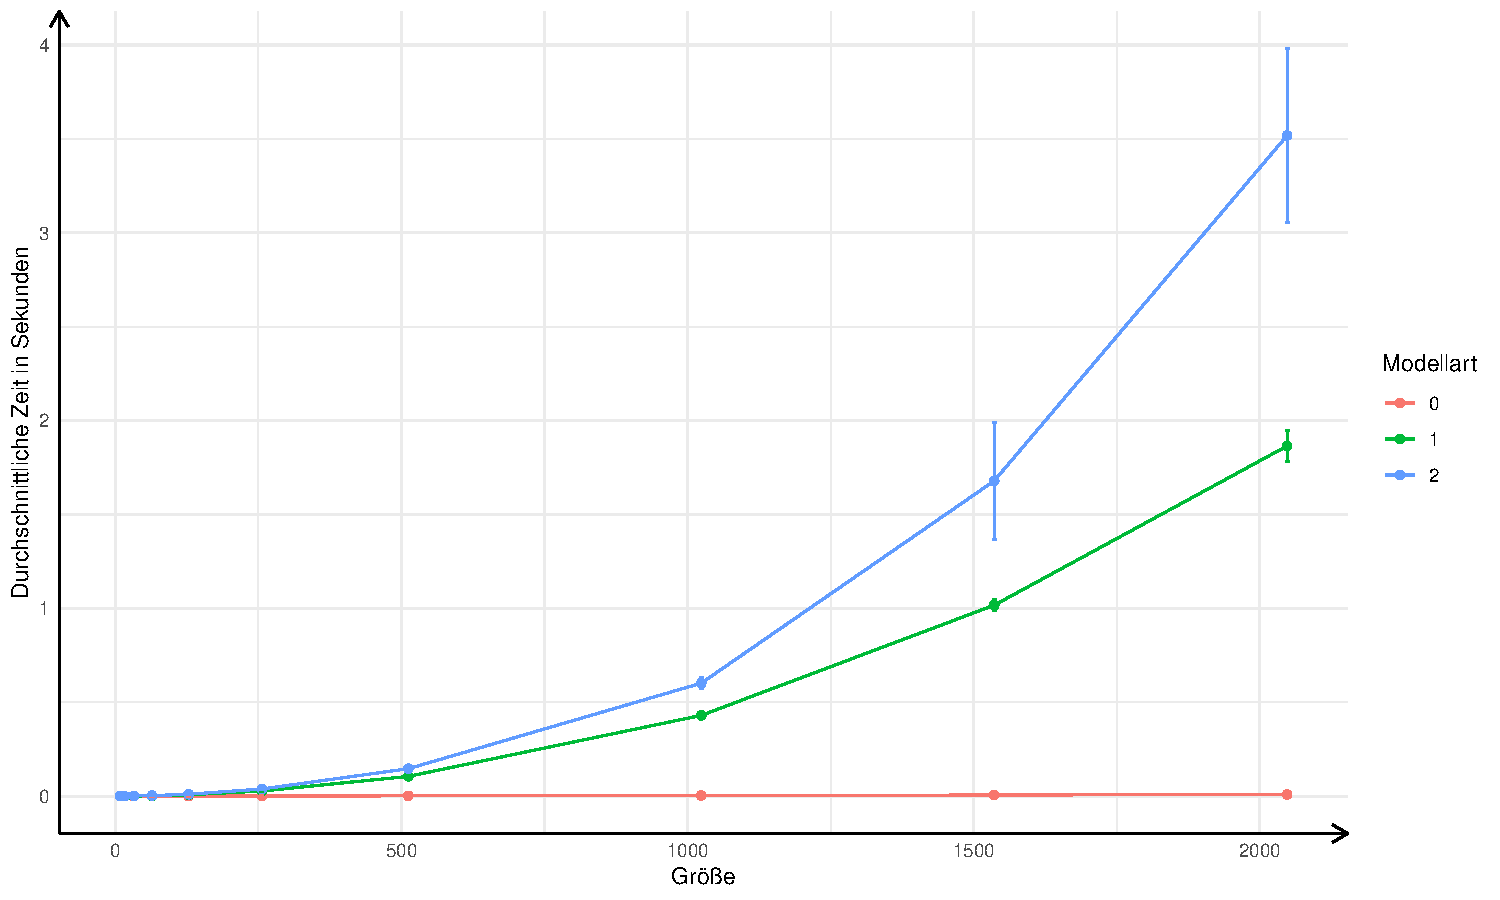
\includegraphics[page=1]{Bilder/pdf/plot_all_release.pdf}}
    \end{center}
\caption{Durchschnittliche Zeit mit 0,99-Konfidenzintervall}\label{fig:messungen_all}
\end{figure}

\section{Profiling Ergebnisse}
\autoref{fig:profiling_art_1} zeigt einen Ausschnitt aus der Profiler-Ausgabe
für das Modell der Art 1 und der Größe 2048. Dieser Ausschnitt beinhaltet dabei
die relevantesten Knoten der Ausgabe. Der \verb+optimize+-Knoten
hat zwar noch weitere Kindknoten. Aufgrund der geringeren Auswirkung auf die
Laufzeit, wurden diese in der Grafik entfernt, um die Übersichtlichkeit zu
erhöhen. Die relevantesten von diesen Knoten werden jedoch im folgenden weiter
betrachtet. Die Ausgabe für Modellart 2 hat einen ähnlichen Aufbau.

\autoref{tab:e_values} stellt für ausgewählte Knoten den Anteil der von
Funktion dieses Knotens benötigten Zeit von der Gesamtzeit dar. Es sind jeweils
alle Messwerte für die verschiedenen Größen angegeben, um auch das Verhalten
analysieren zu können. Diese Werte entsprechen dem in
\autoref{sec:hana_profiler} erläutertem Wert $E$ aus der Profiler-Ausgabe.
Auffällig ist die \verb+opptimize+-Funktion, diese benötigt sowohl bei
Modellart 1 als auch bei Modellart 2 einen sehr großen Anteil der Zeit. Dieser
Anteil steigt jedoch zumindest bei Modellart 2 nicht eindeutig mit der Größe. Dies
bedeutet jedoch nicht, dass die benötigte Zeit in dieser Funktion ebenfalls
nicht steigt, da diese Angaben prozentual zu der jeweiligen Gesamtdauer sind.
Die anderen Knoten sind deshalb interessant, weil der Anteil an der Gesamtdauer
mit der Größe des Modells zunimmt. Die größte Zunahme von Prozentpunkten ist
dabei $32 \% - 19 \% = 13 \%$, die größte prozentuale Steigerung ist
$\frac{12\%}{1,5\%} - 1 = 700\%$. Aufgrund des hohen Anteils oder der großen
Steigerung von diesem bieten sich alle in \autoref{tab:e_values} dargestellten
Funktion für eine nähere Betrachtung an.

\begin{table}[h]
\centering
\resizebox{\textwidth}{!}{
\begin{tabular}{|l|l|c|c|c|c|}
\toprule
\textbf{Art} & \textbf{Funktion} & \textbf{2048} & \textbf{4096} & \textbf{8192} &\textbf{16384} \\
\midrule
1 & Optimizer2::optimize                           & 18 \% & 22 \% & 24 \% & 24 \% \\ \hline
1 & CombineJoinOverProjectionPattern::doesMatch    & 19 \% & 26 \% & 30 \% & 32 \% \\\hline
1 & BuildExpresionFilterPattern::doesMatchInternal & 1,5 \% & 6,1 \% & 11 \% & 12 \% \\\hline
2 & Optimizer2::optimize                           & 37 \% & 32 \% & 33 \% & 34 \% \\ \hline
2 & BuildExpresionFilterPattern::doesMatchInternal & 4,2 \% & 10 \% & 10 \% & 14 \% \\
\bottomrule
\end{tabular}
}
\caption{Anteil an der Gesamtlaufzeit ausgewählter Knoten}\label{tab:e_values}
\end{table}
